\section{Charge Readout Electronics}
\label{sec:studies_electronics}

For a heavy MIP with $\dv{E}{x} \approx \SI{2.1}{\mega\electronvolt\per\centi\metre}$, a \lartpc{} has a charge yield of $\order{\SI{1}{\femto\coulomb\per\milli\metre}}$ as explained in Chapter~\ref{chap:lartpc}.
The readout electronics need to be able to reliably digitise this charge.
This chapter aims to outline the challenges based on present designs and then present several tests of future approaches addressing them.

One of the biggest challenges to detect such low charges is the Signal-to-Noise Ratio (SNR).
Noise can originate from a plethora of sources.
They can be divided into internal, originating inside the electronic components, and pick-up from external sources.

The most important internal source is the \emph{Johnson-Nyquist} noise.
It is generated by the intrinsic motion of the charge carriers at non-zero temperature therefore often called thermal noise.
In statistical thermodynamics, the energy of a system with one degree of freedom,
\begin{IEEEeqnarray}{rCl}
	E & = & \frac{k T}{2} \qc
\end{IEEEeqnarray}
is proportional to its temperature $T$ by the Boltzmann constant $k$.
The stored energy in a capacitor is given by
\begin{IEEEeqnarray}{rCl}
	E & = & \frac{C V ^ 2}{2} \qc
\end{IEEEeqnarray}
where $C$ is capacitance of and $V$ the voltage across the capacitor.
Therefore, the voltage generated by the thermal noise power inside a single capacitor is
\begin{IEEEeqnarray}{rCl}
	V & = & \sqrt{\frac{k T}{C}} \qq*{.}
\end{IEEEeqnarray}
Combining this with the charge in the capacitor,
\begin{IEEEeqnarray}{rCl}
	\label{eq:electronics_thermal-noise}
	Q & = & C V = \sqrt{k T C}
\end{IEEEeqnarray}
is the equivalent noise charge due to the capacitor's temperature.~\cite{noise}

Equation~\eqref{eq:electronics_thermal-noise} has two important consequences for charge detectors: Noise scales with temperature and detector capacitance.
The temperature dependences is one of the main reasons to operate all analogue electronics at cryogenic temperatures.
Due to their much smaller capacitance, noise levels on pixels are significantly lower compared to wires.

Another internal noise source are resonances in the signal path that can start to oscillate.
Resonances can occur from the combination of the impedance of electronic components such as cables and input impedances.
The main culprits are usually parasitic impedances not taken into account during the desing of the circuit.
The resulting oscillations are superimposed on the signal.

An example of such a resonance is the behaviour of the cryogenic LARASIC preamplifiers used for \AT{} and described below.
They include a user configurable shaping filter.
With its change, the input capacitance of the amplifier changes as well.
Some configurations can form resonances with the circuit at the input.
Most passive electronic components change their values more or less significantly with temperature.
Therefore, the resonance behaviour of the detector circuit is different at room temperature and in \lar{}.
Additionally, every deviation from the final setup potentially changes parasitic impedances.
As a result, it is quite challenging to debug such resonances in the signal path.

External sources can induce voltages on the signal path from variable magnetic fields, as predicted by Faraday's law.
Particularly prone to this are ground loops, any closed circuit supposed to be entirely at ground potential.
If the resistance at one place of the loop is high enough, the induction results in a voltage difference along the loop.
If the same part of the loop is used as reference of a signal carrying connection, a difference in the ground reference between signal source and signal sink will affect the signal.

There are several possibilities to make a circuit more resilient to external noise sources.
An obvious one is shielding all sensitive parts from external magnetic fields using a Faraday cage.
Implementing this effectively is extremely complicated and often not practical for small experiments.
Another approach is hardening the signal path itself by using current-coupled and/or symmetric signals.
Current-coupled signals are much less sensitive to induced voltages, as long as they are small enough and do not result in significant current across parasitic impedances.
An example is NIM logic from the Nuclear Instrumentation Module standard.

\begin{figure}[htb]
	\centering
	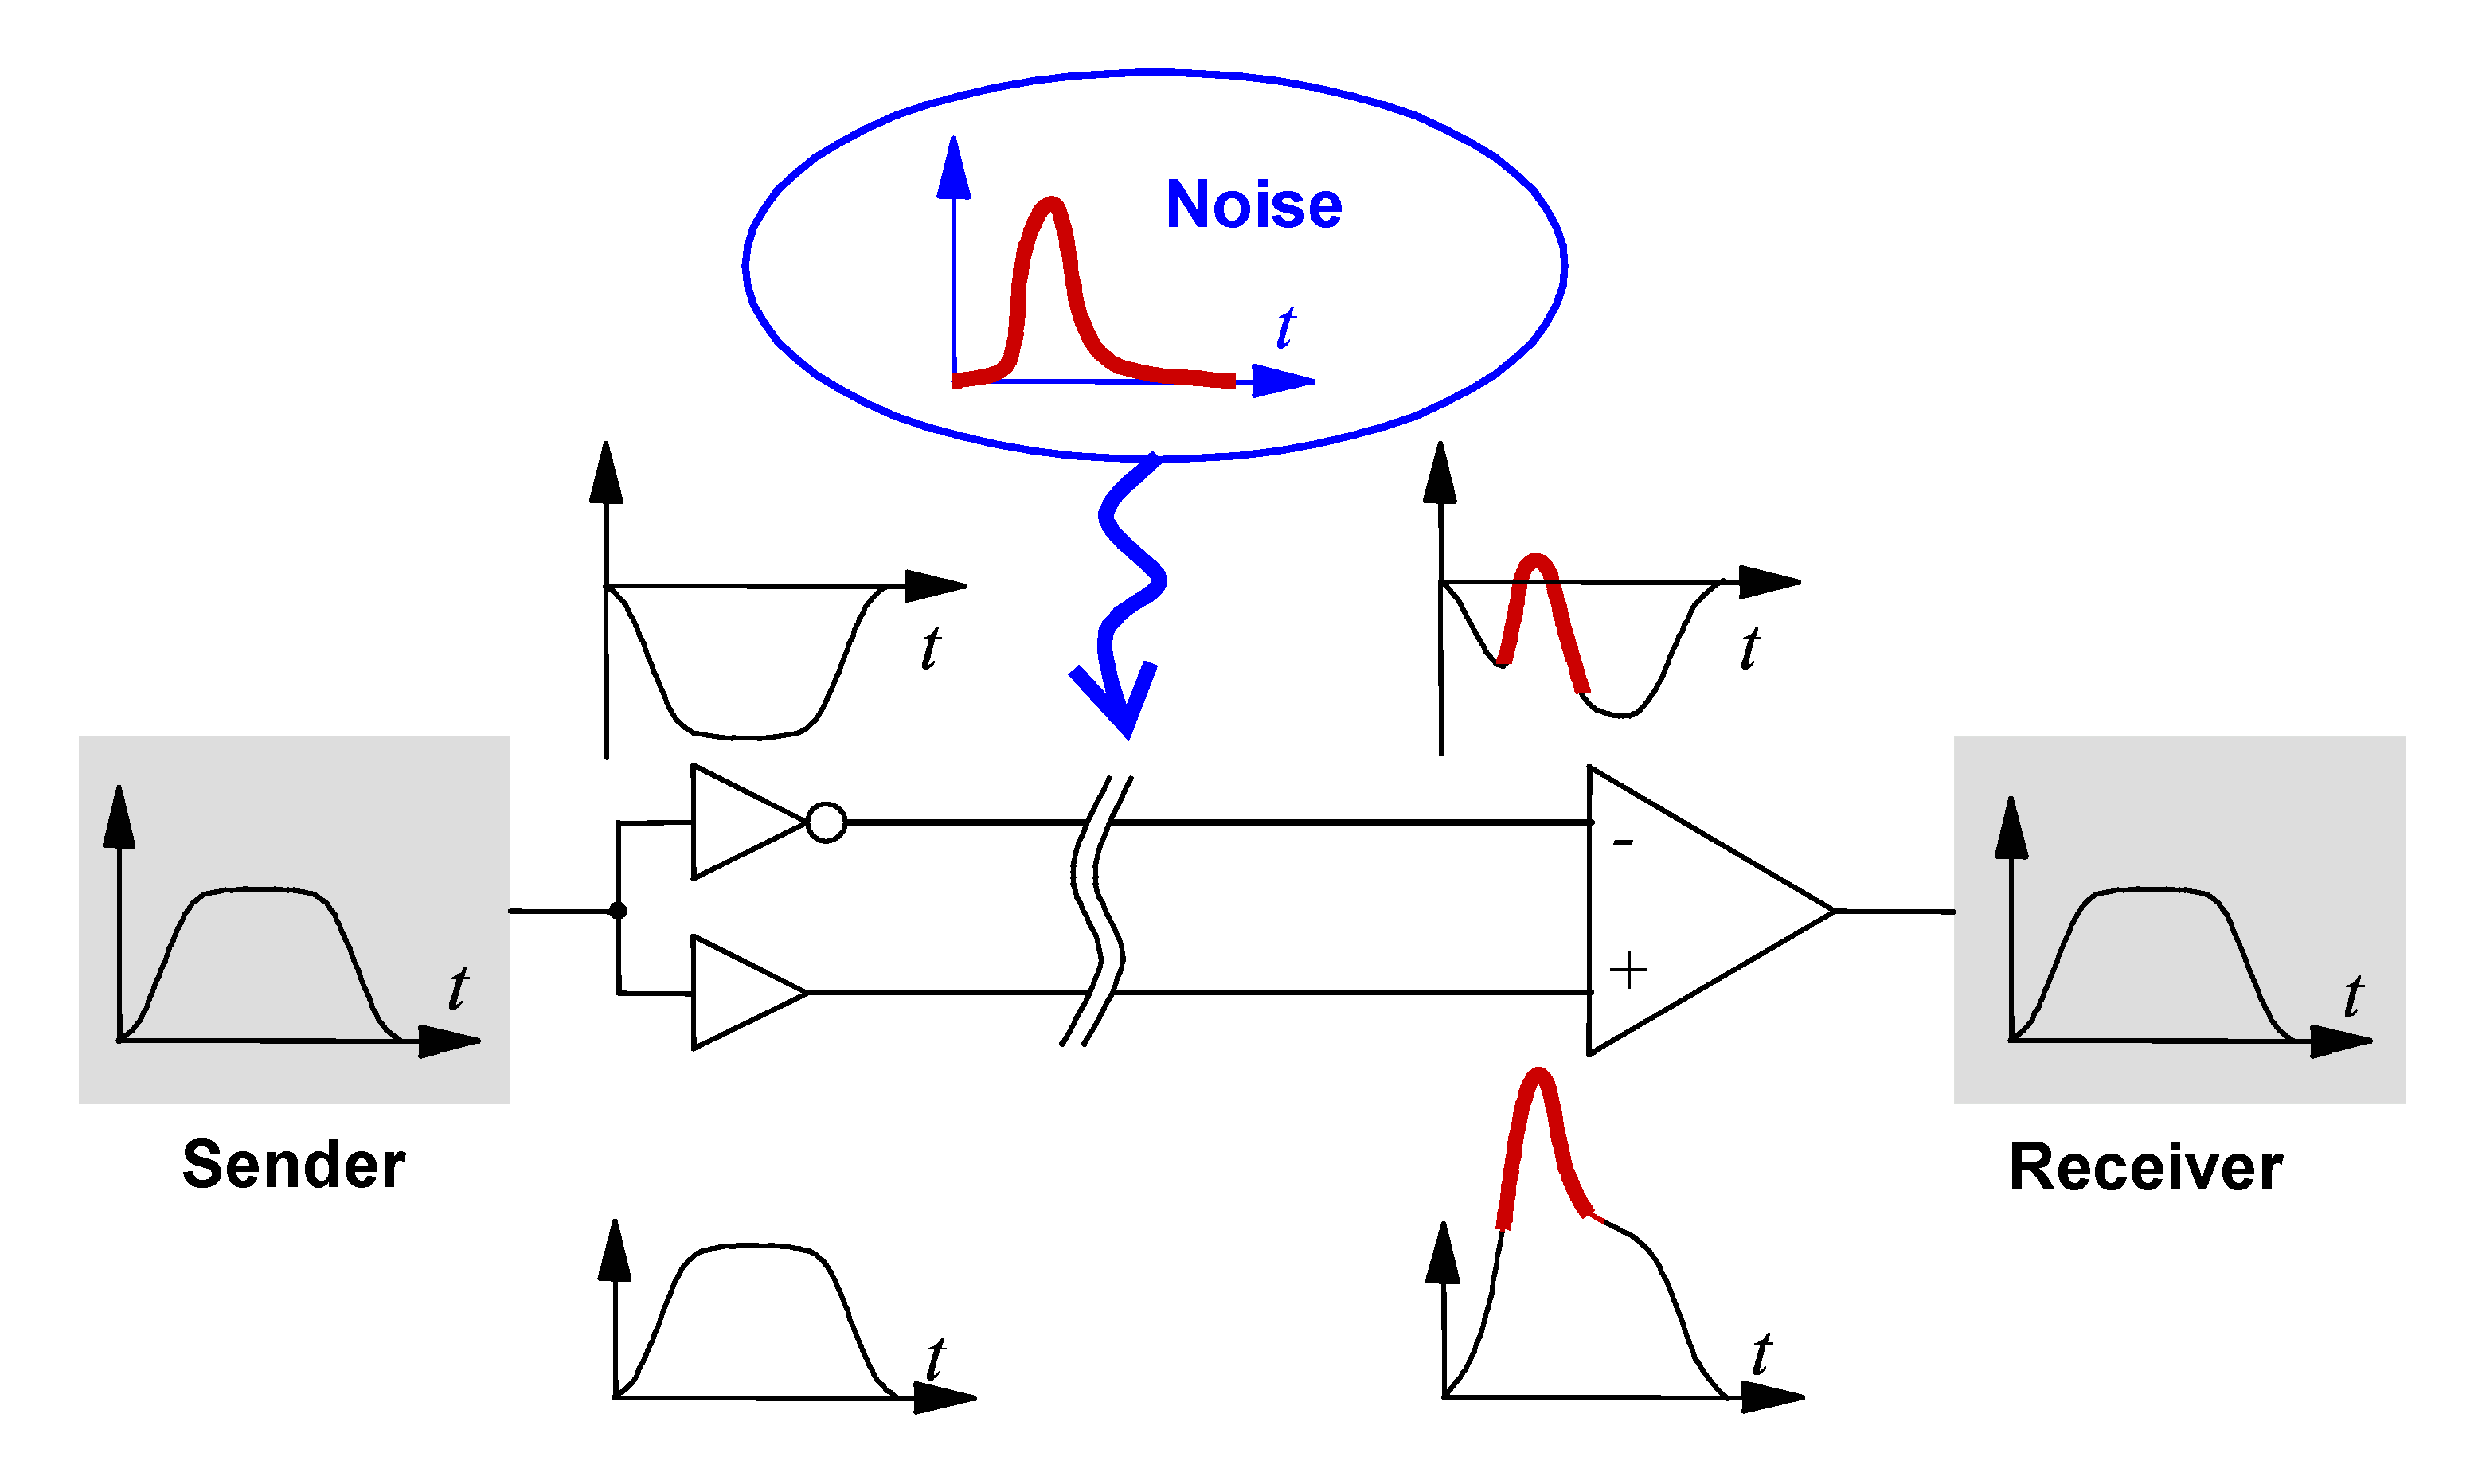
\includegraphics[width=\textwidth]{electronics/DiffSignaling}
	\caption{Noise reduction using differential signalling.~\cite{diff_signal}}
	\label{fig:electronics_diff-signal}
\end{figure}

For conventional single-ended signalling, the signal is measured as the voltage or current difference between a signal conductor and a ground common to the signal source and the signal sink.
Using a common ground as signal return path can have several undesired effects.
To shield the signal conductor, it is usually enclosed in a ground shield.
If the latter is connected on both sides, a ground loop can result for instance in combination with a shared power supply ground.
Ground loops can pick up noise through induction if the resistance along the loop is high enough.
A second way to couple noise into a single-ended system is by shifting the potential on the common ground away from the reference voltage or current, for instance due to high currents flowing through a lossy ground connection.
Because the signal is always measured against the common ground, it will be distorted.
In symmetric or differential signalling, the signal is not measured between a signal conductor and ground but instead between two signal conductors.
This works by putting an inverted (symmetric) waveform of the signal on a second conductor.
The signal is recovered by taking the difference between to two signal conductors.
As a result, the signal sink needs not be connected to the same ground as the signal source because the signal is independent of ground.
Ground loops can thus be avoided in the signal path.
Furthermore, the effects of noise pick-up on the signal lines is drastically reduced.
Due to the completely symmetric signal path, inductive noise pick-up is equal on both signal conductors as opposed to single-ended signals where the signal path is not symmetric.
In the signal sink, the difference between the two symmetric signal conductors is formed and everything that is present on both of them, such as the inductively picked up noise, cancels out.

Disentangling the three different sources of noise (thermal noise, resonances, and external pick-up) is not easy.
Hints can often be found in the spectrum of the noise.
Thermal noise is equal and uncorrelated over the full frequency spectrum.
Resonances usually occur at specific frequencies and thus produce regular patterns such as a sine at the resonance frequency.
External sources are more difficult to identify.
If the source produces electromagnetic fields at known frequencies (e.g.\ harmonics of a switched power supply) the noise spectrum can be scanned for these.
On the other hand if the source is unknown, debugging is much more complex.


\subsection*{\AT Chain}

Contemporary electronics schemes shall be introduced by looking at the existing readout chain at LHEP at the University of Bern.
It was originally designed for the \AT{} experiment and a more detailed description can be found in~\cite{AT_larasic}.

The charge collected by the readout plane is amplified by LARASIC4*~\cite{larasic} cryogenic charge amplifiers developed by Brookhaven National Laboratory (BNL) for \uboone{}~\cite{uboone}.
A performance characterisation of these application-specific integrated circuits (ASICs) can be found in~\cite{AT_larasic}.
Their main features include

\begin{itemize}
	\item \num{16} channels per ASIC;
	\item low noise charge amplifiers incorporating high-order filters;
	\item per channel programmable gain of \SIlist[list-final-separator = { or }]{4.7; 7.8; 14; 25}{\milli\volt\per\femto\coulomb};
	\item per channel programmable filter peaking time of \SIlist[list-final-separator = { or }]{0.5; 1.0; 2.0; 3.0}{\micro\second};
	\item built-in test capacitance connected to dedicated external test pulse input for calibration;
	\item and a power dissipation \SI{< 10}{\milli\watt} per channel.
\end{itemize}

\begin{figure}[htb]
	\centering
	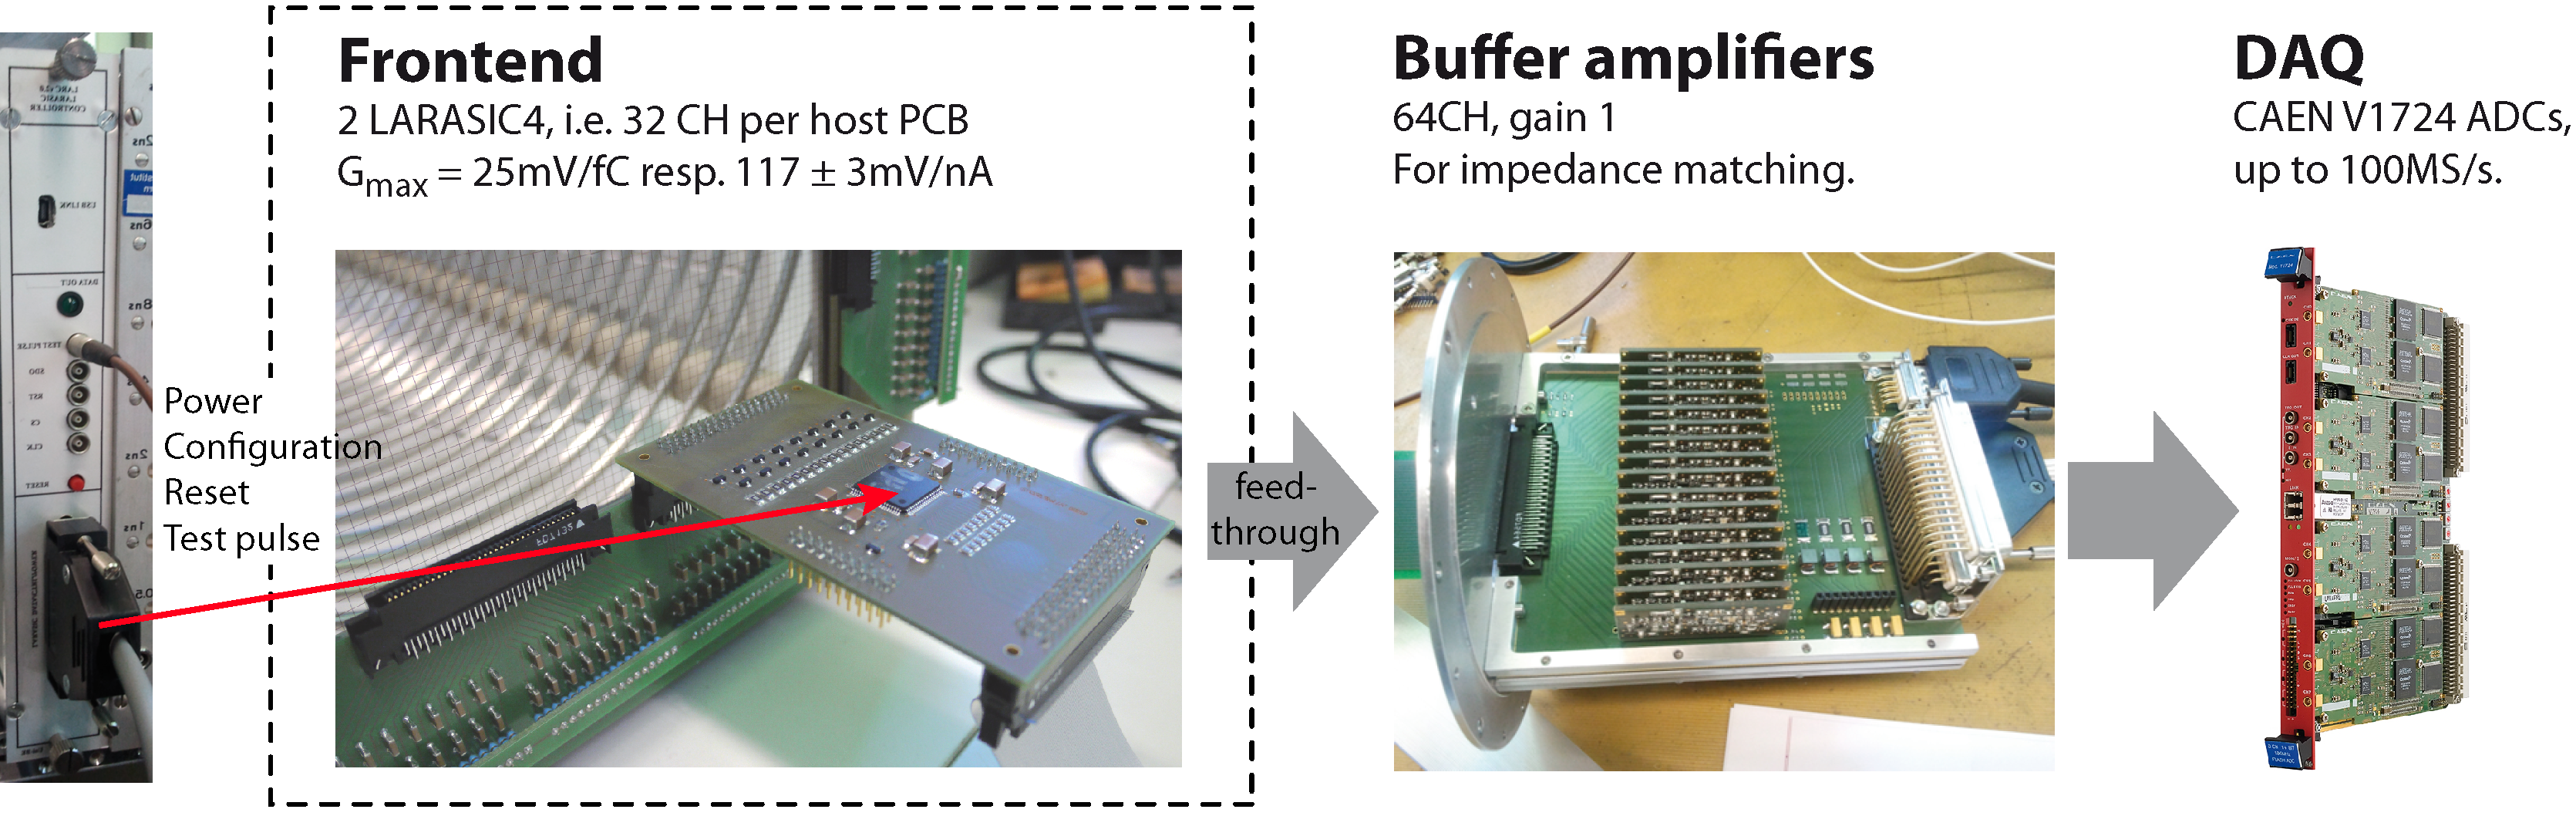
\includegraphics[width=\textwidth]{electronics/ReadoutChain_AT}
	\caption{Readout chain used for the pixel test.
		The picture of the LARASIC cryogenic front-end preamplifiers shows them installed in the \AT{} wire readout setup.~\cite{AT_larasic}}
	\label{fig:viper_readoutChain_AT}
\end{figure}

The cryogenic preamplifiers are mounted as close as possible to the readout in order to minimise noise pick-up on these very sensitive lines.
Via an inter-integrated circuit (I\textsuperscript{2}C) bus, LARASICs can be programmed to the different aforementioned configurations.
For this purpose, they are connected to a bespoke NIM module housing an Arduino which generates the I\textsuperscript{2}C signals, a test pulse generator, and multiple low-noise voltage regulators providing power to the LARASICs.
The output of the preamplifiers is fed to buffer amplifiers mounted on top of the signal feedthrough by means of flexible Kapton ribbon cables.
The buffers operate at room temperature, have a unity gain, and match the output impedance of the LARASICs to the \SI{50}{\ohm} input impedance of the downstream digitisers.
From the buffers, the signals are routed via \SI{50}{\ohm} unbalanced coaxial lines to \emph{CAEN V1724}\footnote{\url{http://www.caen.it}} \SI{14}{bit} digitisers mounted in a VME crate.
For debugging purposes, the output of the buffers can be routed to an oscilloscope via a coaxial T-piece.
Finally, the digital data is read out from the VME crate via a fibre-optic link by a standard PC.
Figure~\ref{fig:viper_readoutChain_AT} depicts the entire readout chain.
The complete analogue signal path from the pixel plane to the VME digitisers is single-ended and thus prone to ground loops and all associated noise problems.

\begin{figure}[htb]
	\centering
	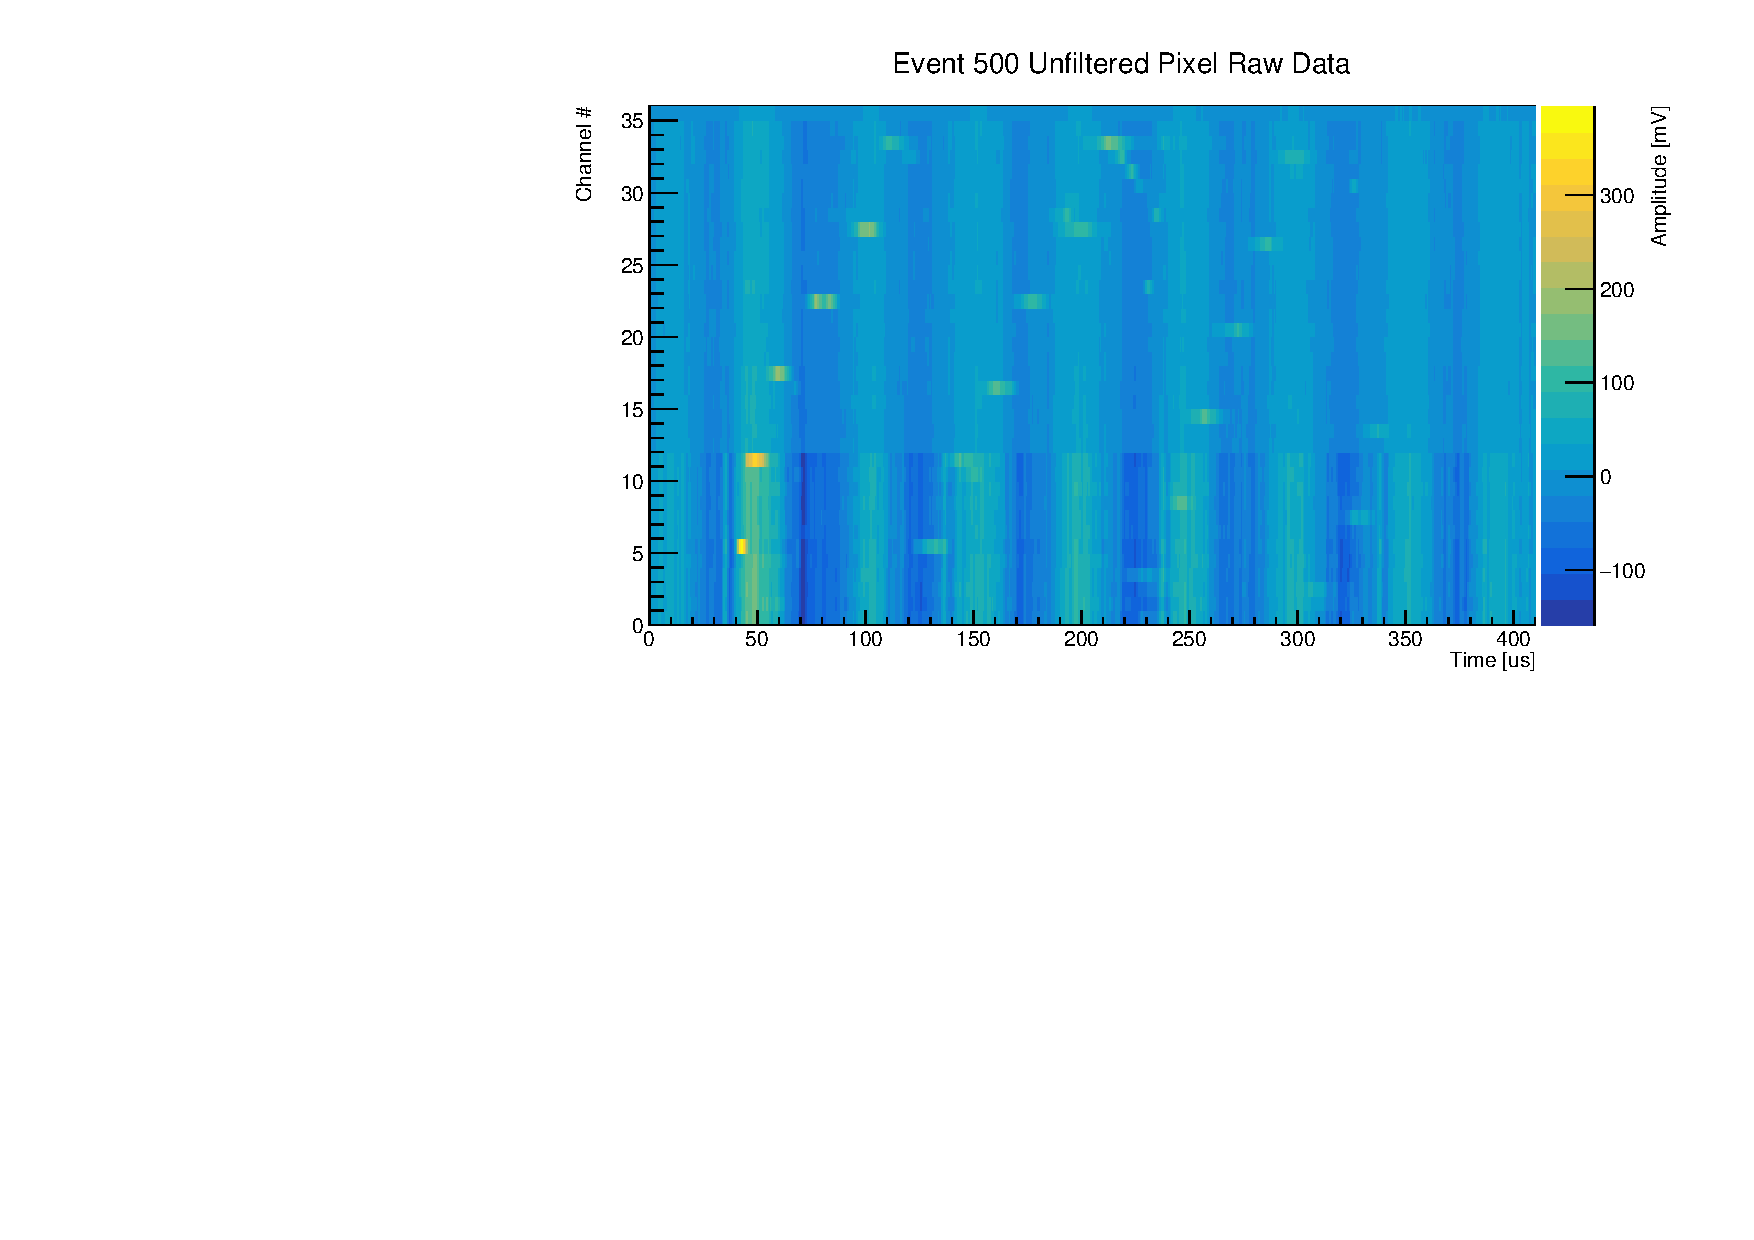
\includegraphics[width=\textwidth]{noise/event500_rawUnfilteredPixel}\\
	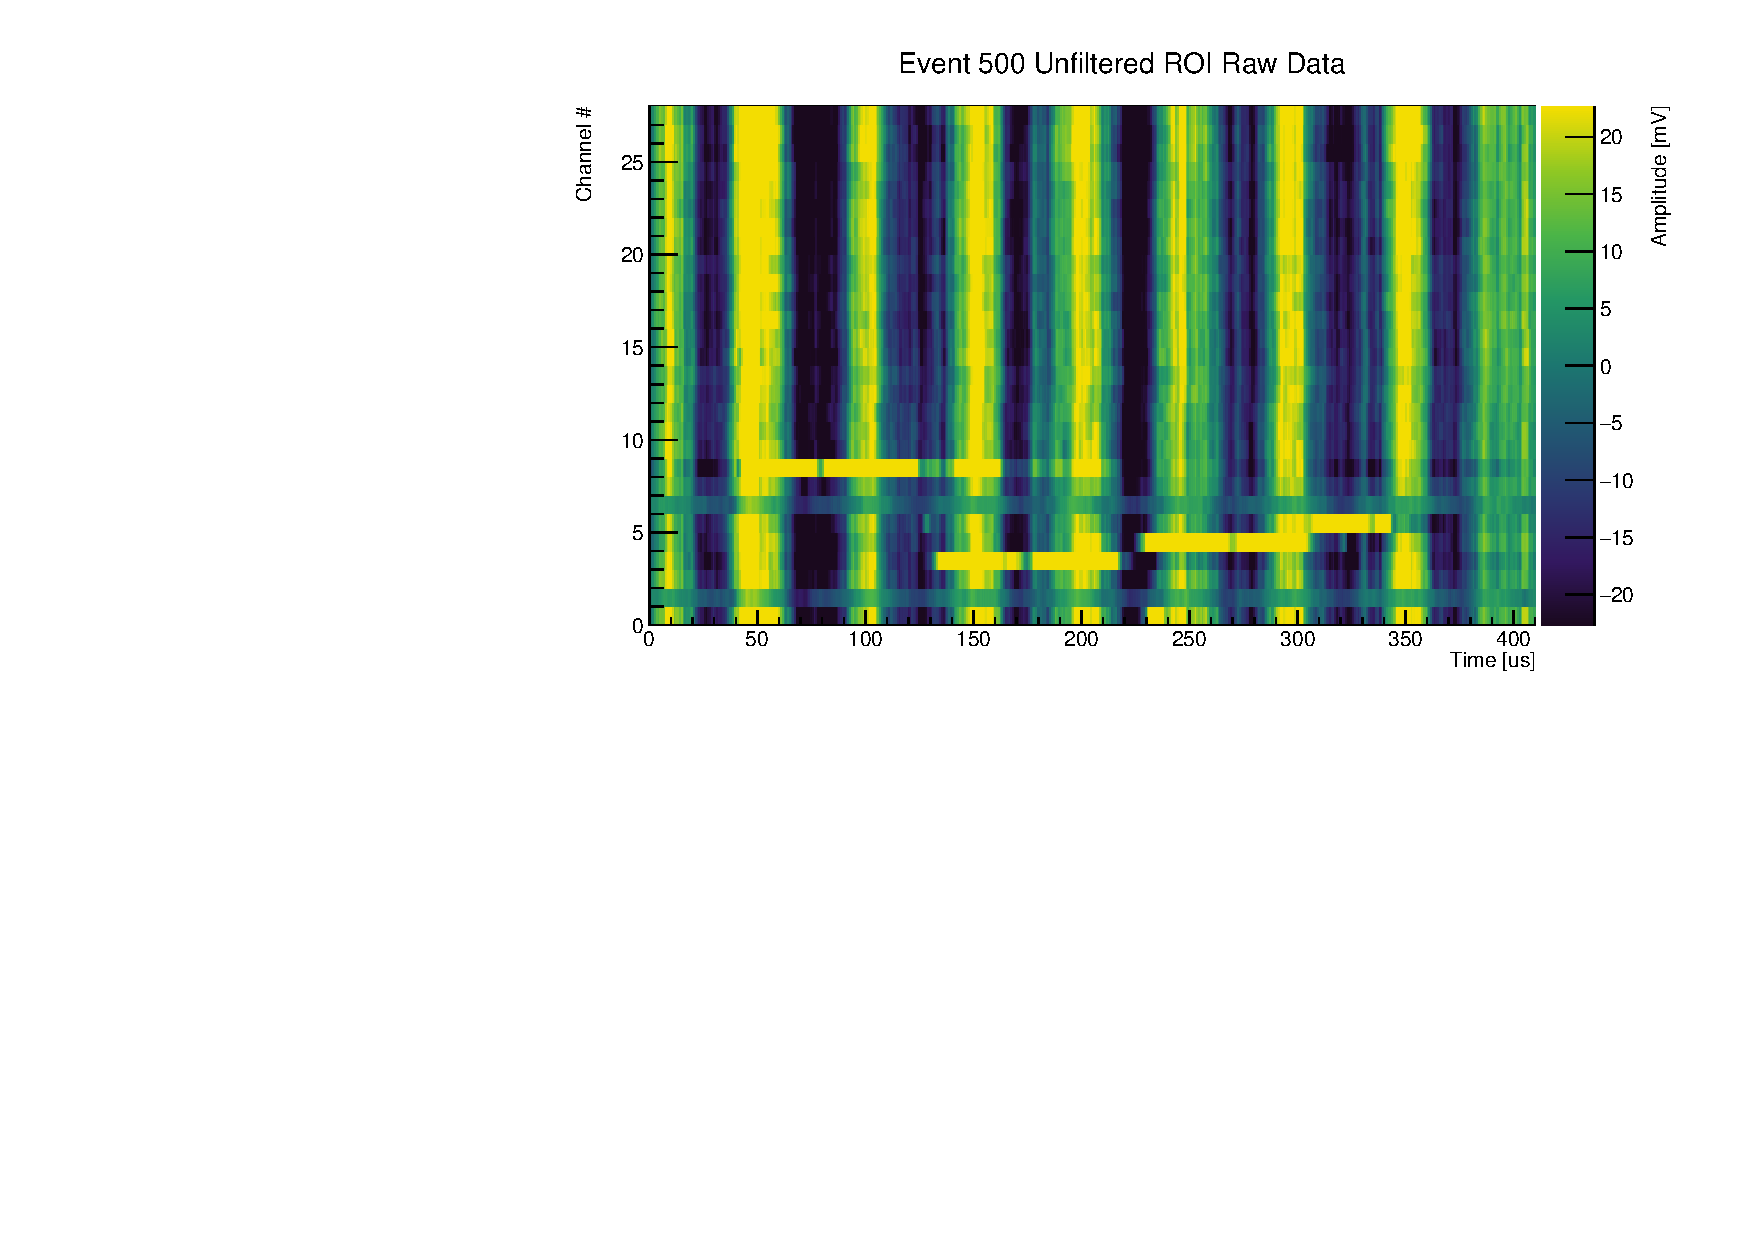
\includegraphics[width=\textwidth]{noise/event500_rawUnfilteredROI}
	\caption{Event from the first measurement campaign of the pixel prototype.
	The top plot shows pixel data while the bottom plot shows ROI data.}
	\label{fig:electronics_event-run1}
\end{figure}

During the first pixelated readout measurement campaign (see Sections~\ref{sec:studies_charge-ro} and~\ref{sec:ac_viper}), it became apparent that the data was significantly impaired by noise.
As can be seen in Figure~\ref{fig:electronics_event-run1}, the noise amplitude is similar over multiple channels.
This implies a common mode component that cannot originate from inductive pick-up.
Instead, the noise is likely generated by self-oscillating parts of the signal path due to ground loops and parasitic impedances.
For the second measurement campaign, different steps were take to mitigate this behaviour through modifications to detector location, power supply, signal path, and intrinsic capacitance.

A correlation between noise levels and the running state of the air condition in the utility room next to the lab was found.
Therefore, the experimental setup was moved away from the wall facing the utility room.

A decoupled clean power grid was built in the lab.
A Motor Generator (M-G set) separates the lab grid mechanically from the building power supply.
Thus, any noise present on the latter is prevented from entering the experimental setup.
Furthermore, this decouples the lab grid entirely from the building ground preventing ground loops via electric mains.

\begin{figure}[htb]
	\centering
	\includegraphics[page=4, width=\textwidth]{noise/noise_run1} \\
	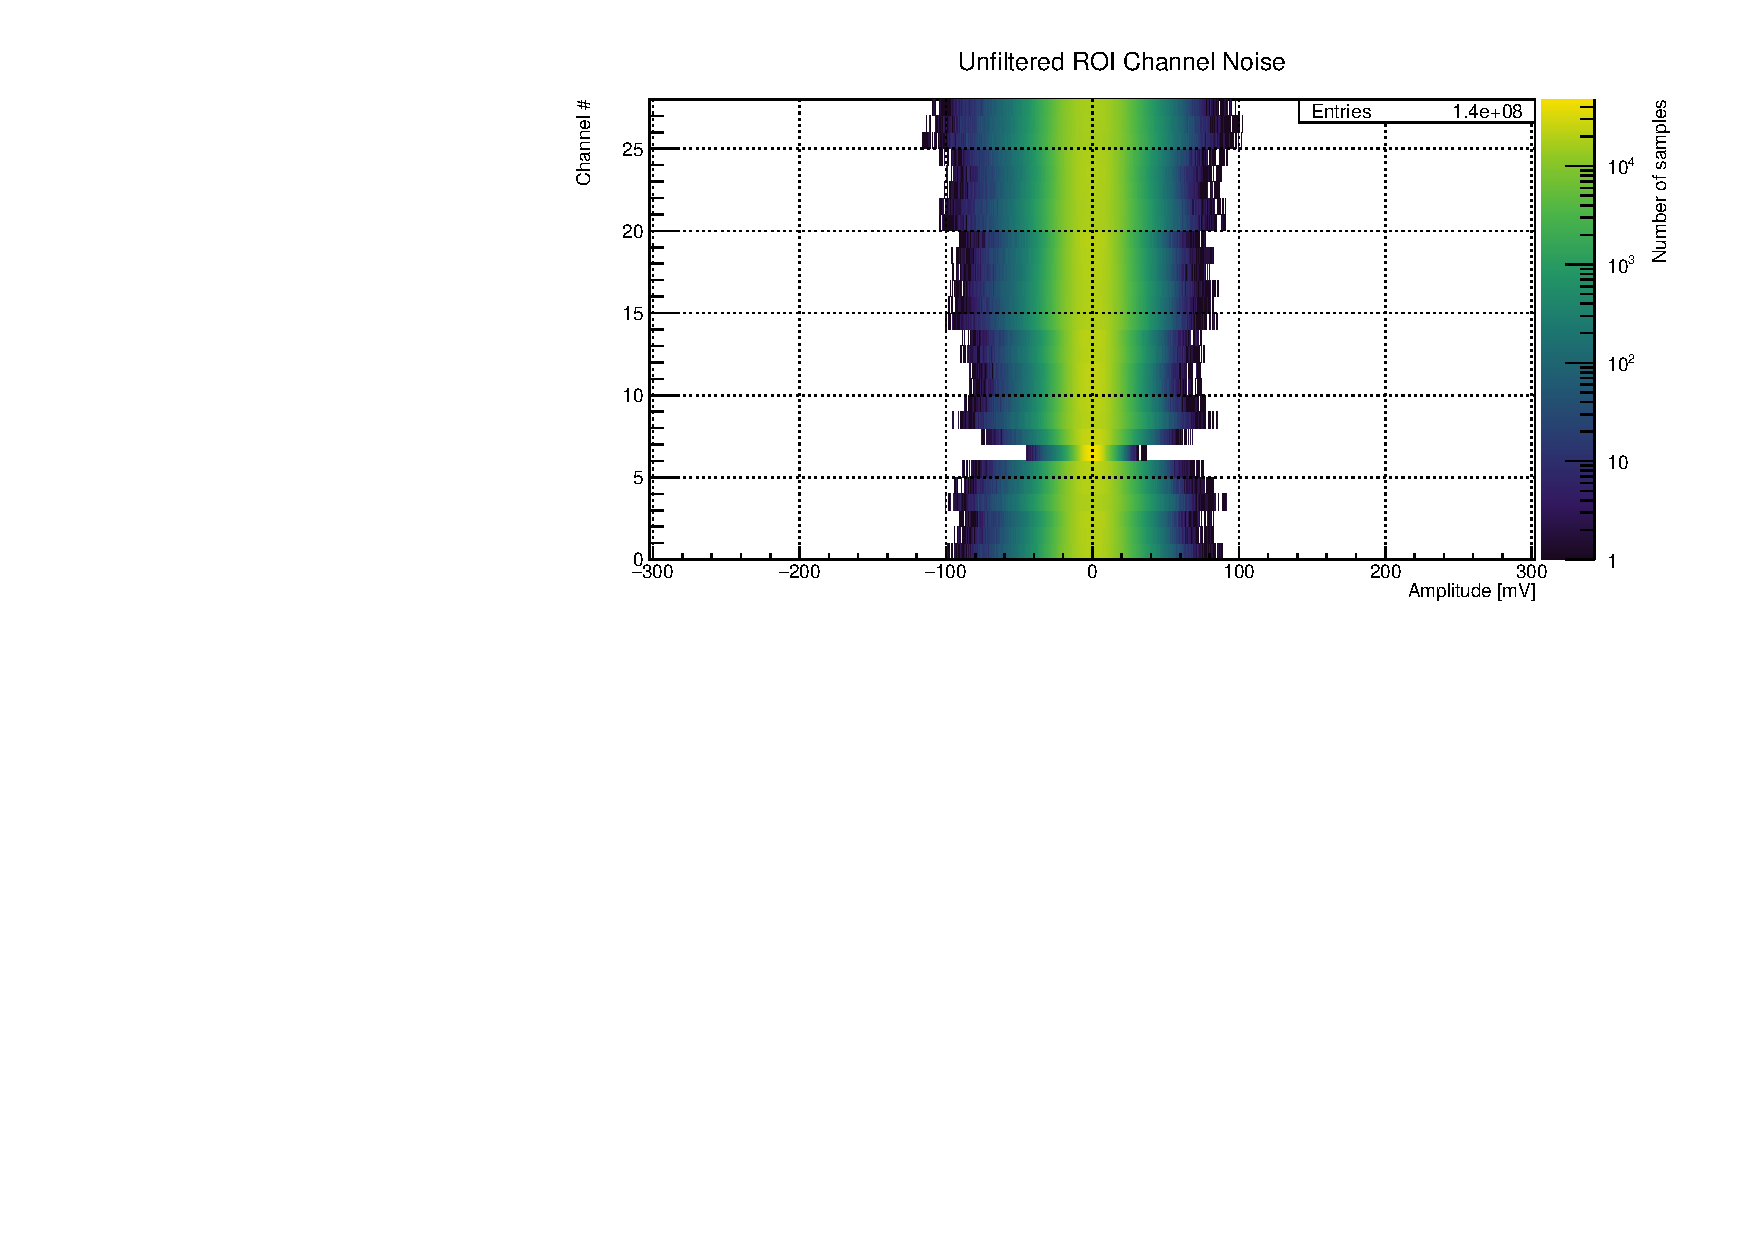
\includegraphics[page=1, width=\textwidth]{noise/noise_run1}
	\caption{Noise amplitude distributions of pixel (top) and ROI (bottom) channels of the first measurement campaign.
	\num{5000} events with \num{1000} \SI{410}{\nano\second} samples each from a \SI{5}{\hertz} random trigger were combined.}
	\label{fig:electronics_noise-run1}
\end{figure}

The signal path from the impedance-matching buffer amplifiers to the digitisers---i.e. the warm signal path---was changed from single-ended to differential signalling.
This was achieved by replacing the buffer amplifiers by single-ended to differential amplifiers and inserting another stage upstream of the digitisers to change the signal back to \SI{50}{\ohm} single-ended, matching the input of the digitisers.
Like this, noise pick-up outside the cryostat could be reduced as well as sensitivity to ground loops between the detector and the DAQ rack.
The design for the two buffer stages was kindly provided by the \lariat{} collaboration (see Section~\ref{sec:ac_pixlar} and~\cite{lariat}).

\begin{figure}[htb]
	\centering
	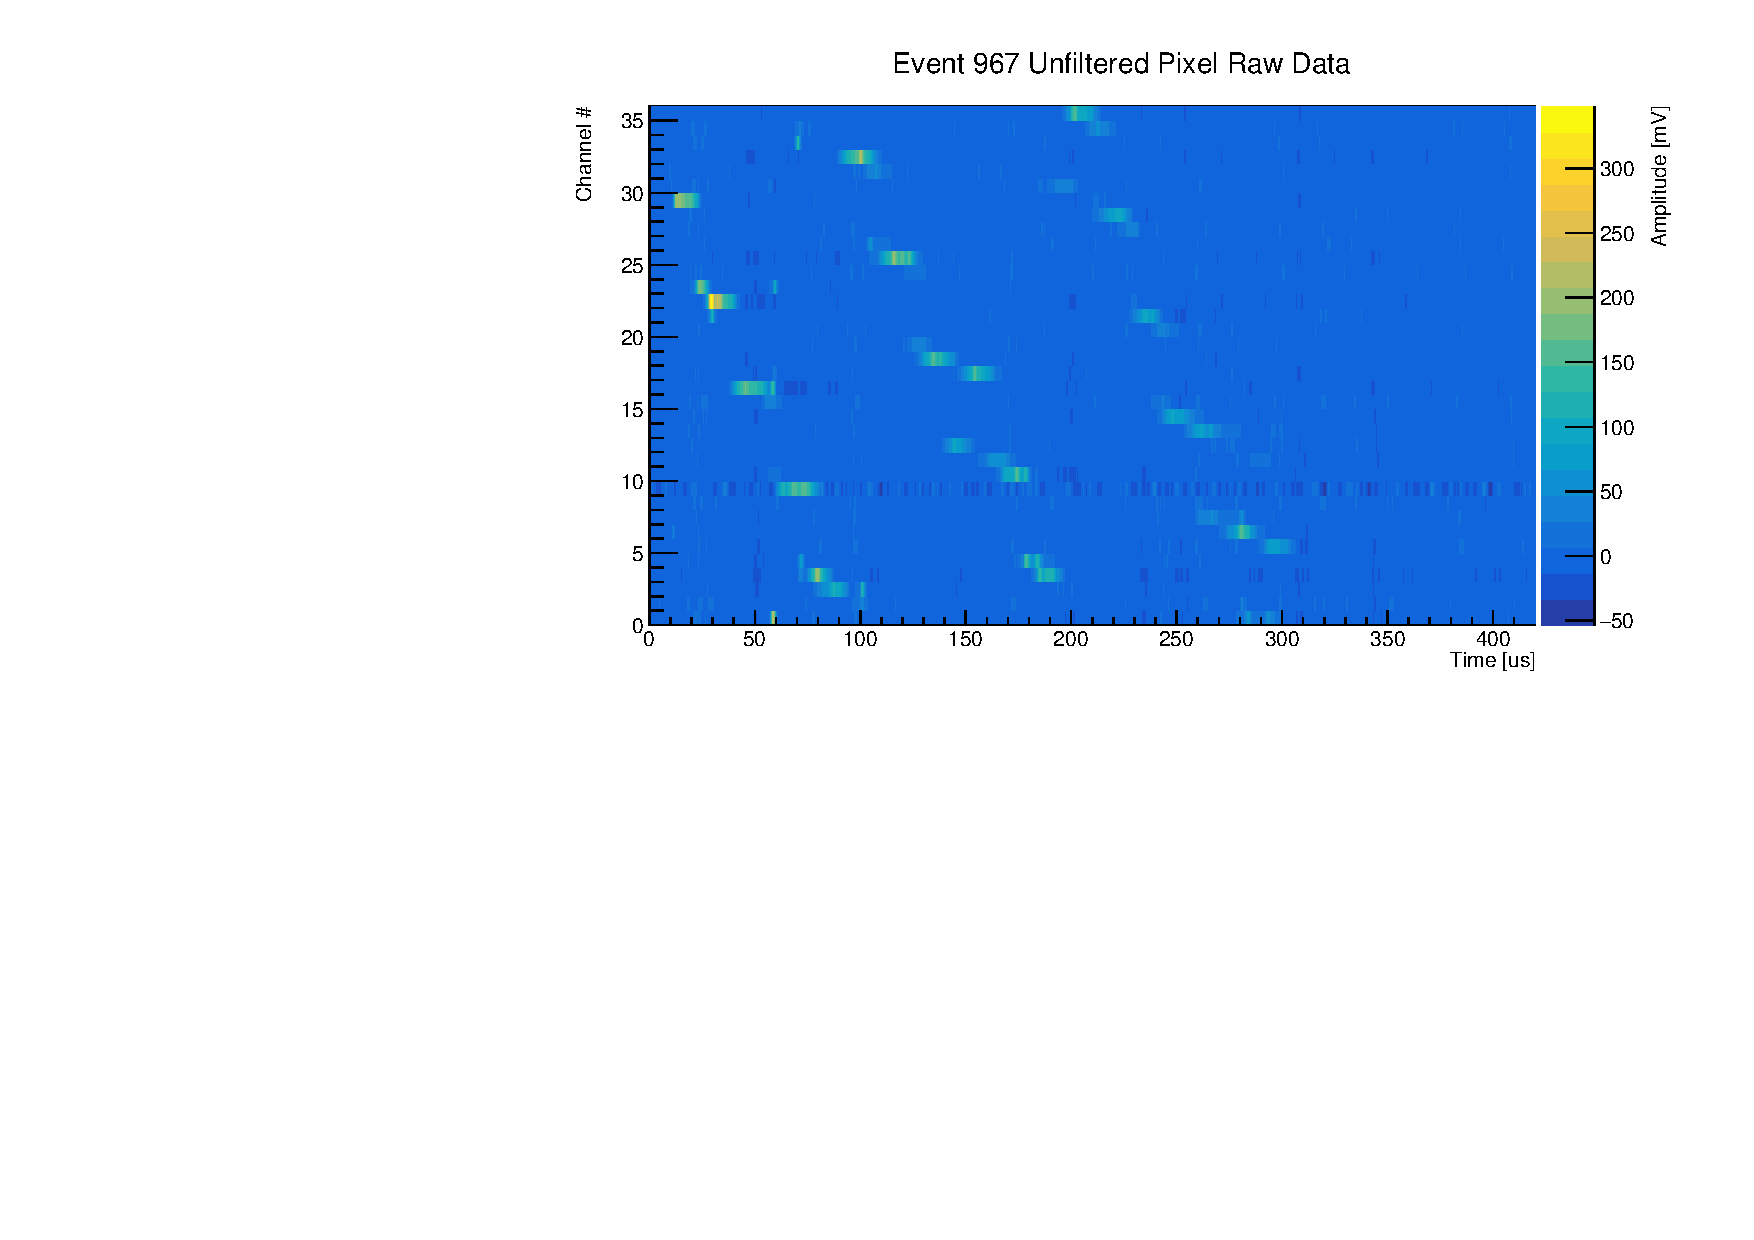
\includegraphics[width=\textwidth]{viper/event967_rawUnfilteredPixel}\\
	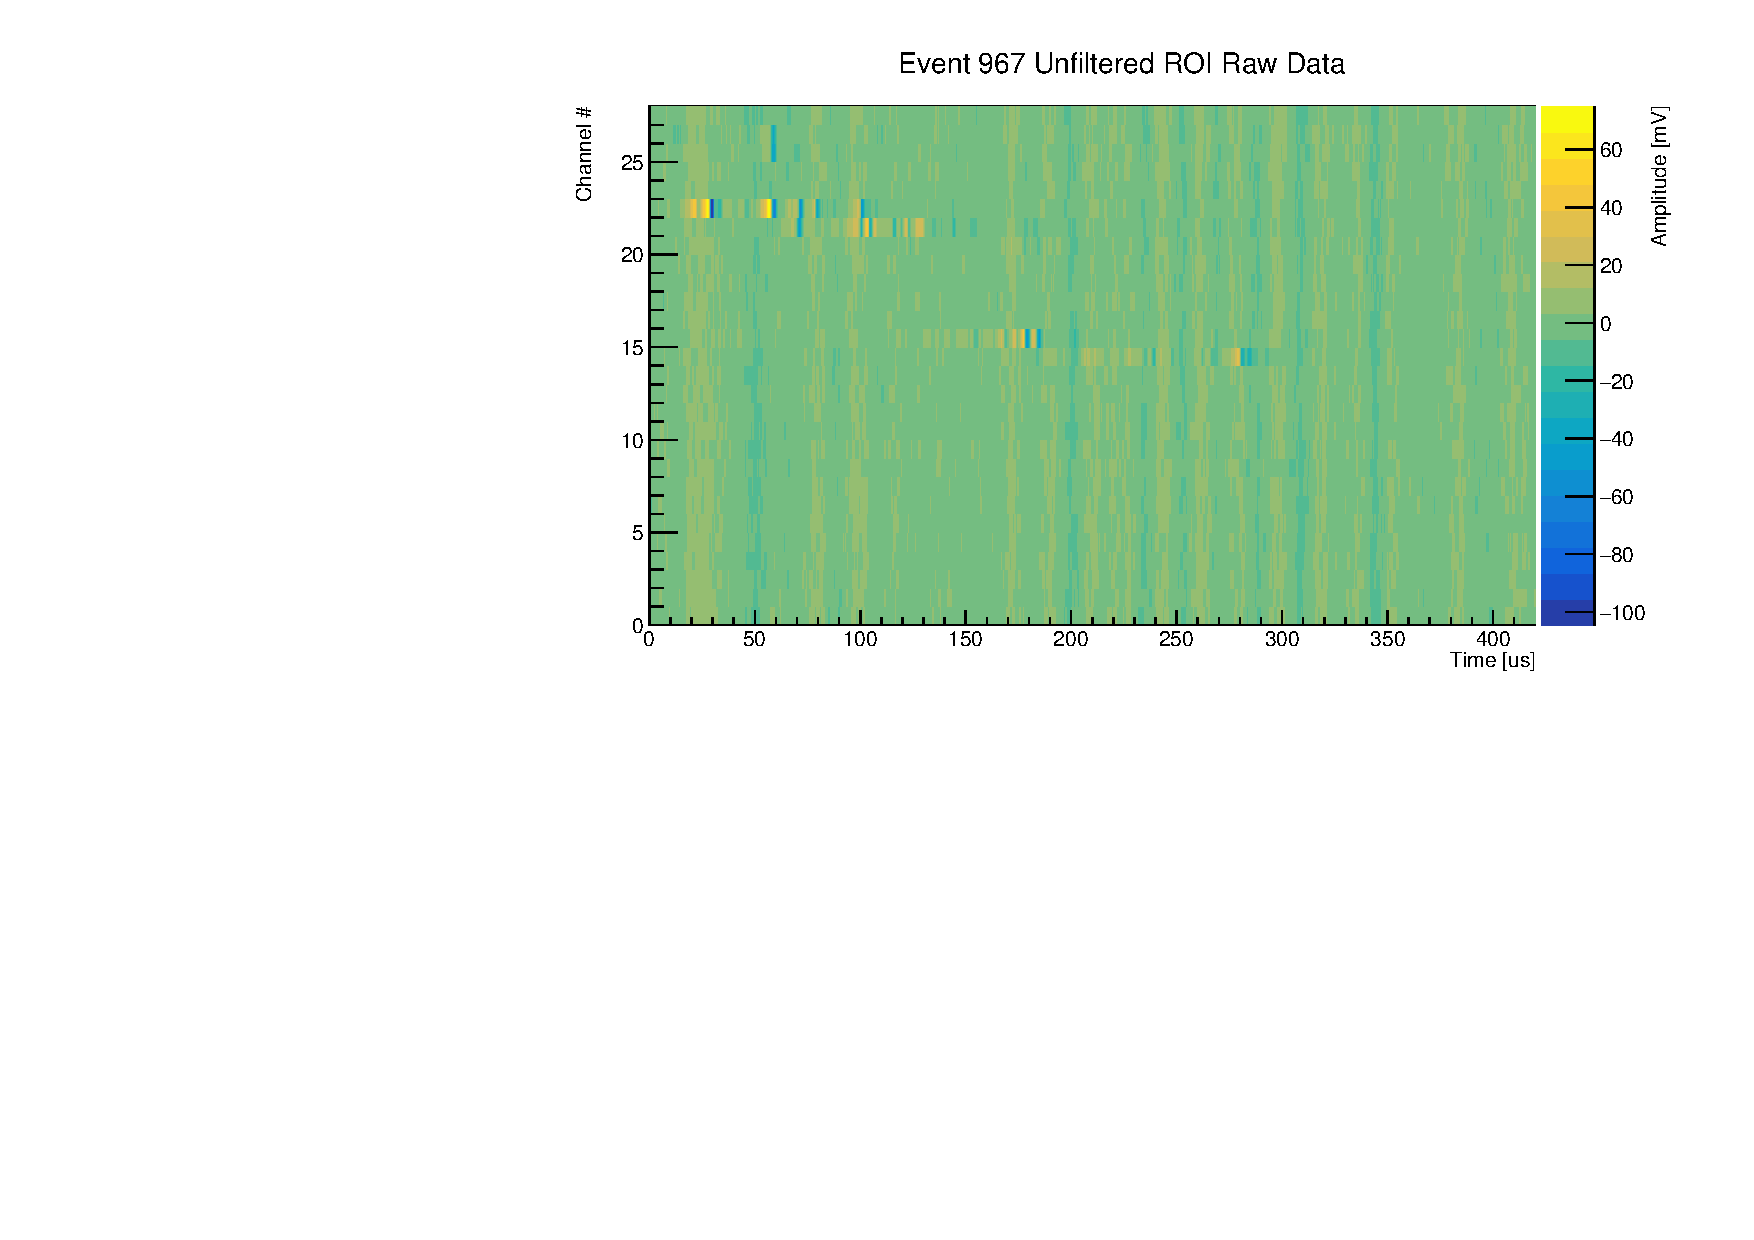
\includegraphics[width=\textwidth]{viper/event967_rawUnfilteredROI}
	\caption{Event from the second measurement campaign of the pixel prototype after improving the readout chain.
	The top plot shows pixel data while the bottom plot shows ROI data.}
	\label{fig:electronics_event-run2}
\end{figure}

A source of noise was identified in the layout of the pixel readout plane.
It was found that due to several ground planes and long tracks in the PCB, parasitic capacitances are very high.
Pixel channels are affected particularly due to the increased total track lengths from connecting multiple pixels to the same DAQ channel.
This is problematic because for high enough frequencies---determined by $RC$---, the input is shorted to ground creating a ground loop again.
Through this capacitive coupling to ground, the system can start to oscillate.
One evidence for this is that the noise is equal over multiple channels, so-called common-mode noise.
More specifically, the noise is equal for two respective groups of channels (see Figure~\ref{fig:electronics_event-run1}).
Investigating this, it was found that these groups correspond to channels of roughly equal parasitic capacitance: \SI{150 +- 5}{\pico\farad} and \SI{95 +- 5}{\pico\farad}.
The noise amplitude is higher on channels with higher capacitance (see Figure~\ref{fig:electronics_noise-run1}).
To solve this problem, the PCB design was optimised by removing unnecessary ground planes, routing signal tracks outside necessary ground planes and increasing the thickness of the PCB.
Pixel capacitance could be improved to \SI{65 +- 5}{\pico\farad} for all channels.
ROI capacitance improved only slightly from \SI{25 +- 10}{\pico\farad} to \SI{20 +- 10}{\pico\farad} which confirms the hypothesis that the long tracks due to pixel multiplexing were the culprits.
The reason for the higher spread of the ROI capacitances is the larger difference in track length between the differen ROIs.
For the sake of completeness, it should be noted here that for the capacitance measurements, the old PCB was not populated while the new one was populated as described in Section~\ref{sec:ac_viper}.
However, the installed capacitors are either not connected to ground or in series with a \SI{10}{\mega\ohm} resistor.
Therefore, their influence on the measurements is negligible.

As can be seen from Figures~\ref{fig:electronics_event-run1} and~\ref{fig:electronics_event-run2}, there is a significant decrease in noise after commissioning all of the above improvements to the readout chain.
This can also be seen from Figures~\ref{fig:electronics_noise-run1} and~\ref{fig:electronics_noise-run2} depicting the noise amplitude distribution of the two measurement campaigns.
The data for the latter (\num{5000} events in the first and \num{2000} events in the second campaign) was taken employing a \SI{5}{\hertz} random trigger.
A more detailed assessment of the noise after the implementation of the described noise mitigation measures can be found in Section~\ref{sec:ac_viper}.

\begin{figure}[htb]
	\centering
	\includegraphics[page=4, width=\textwidth]{noise/noise_run2} \\
	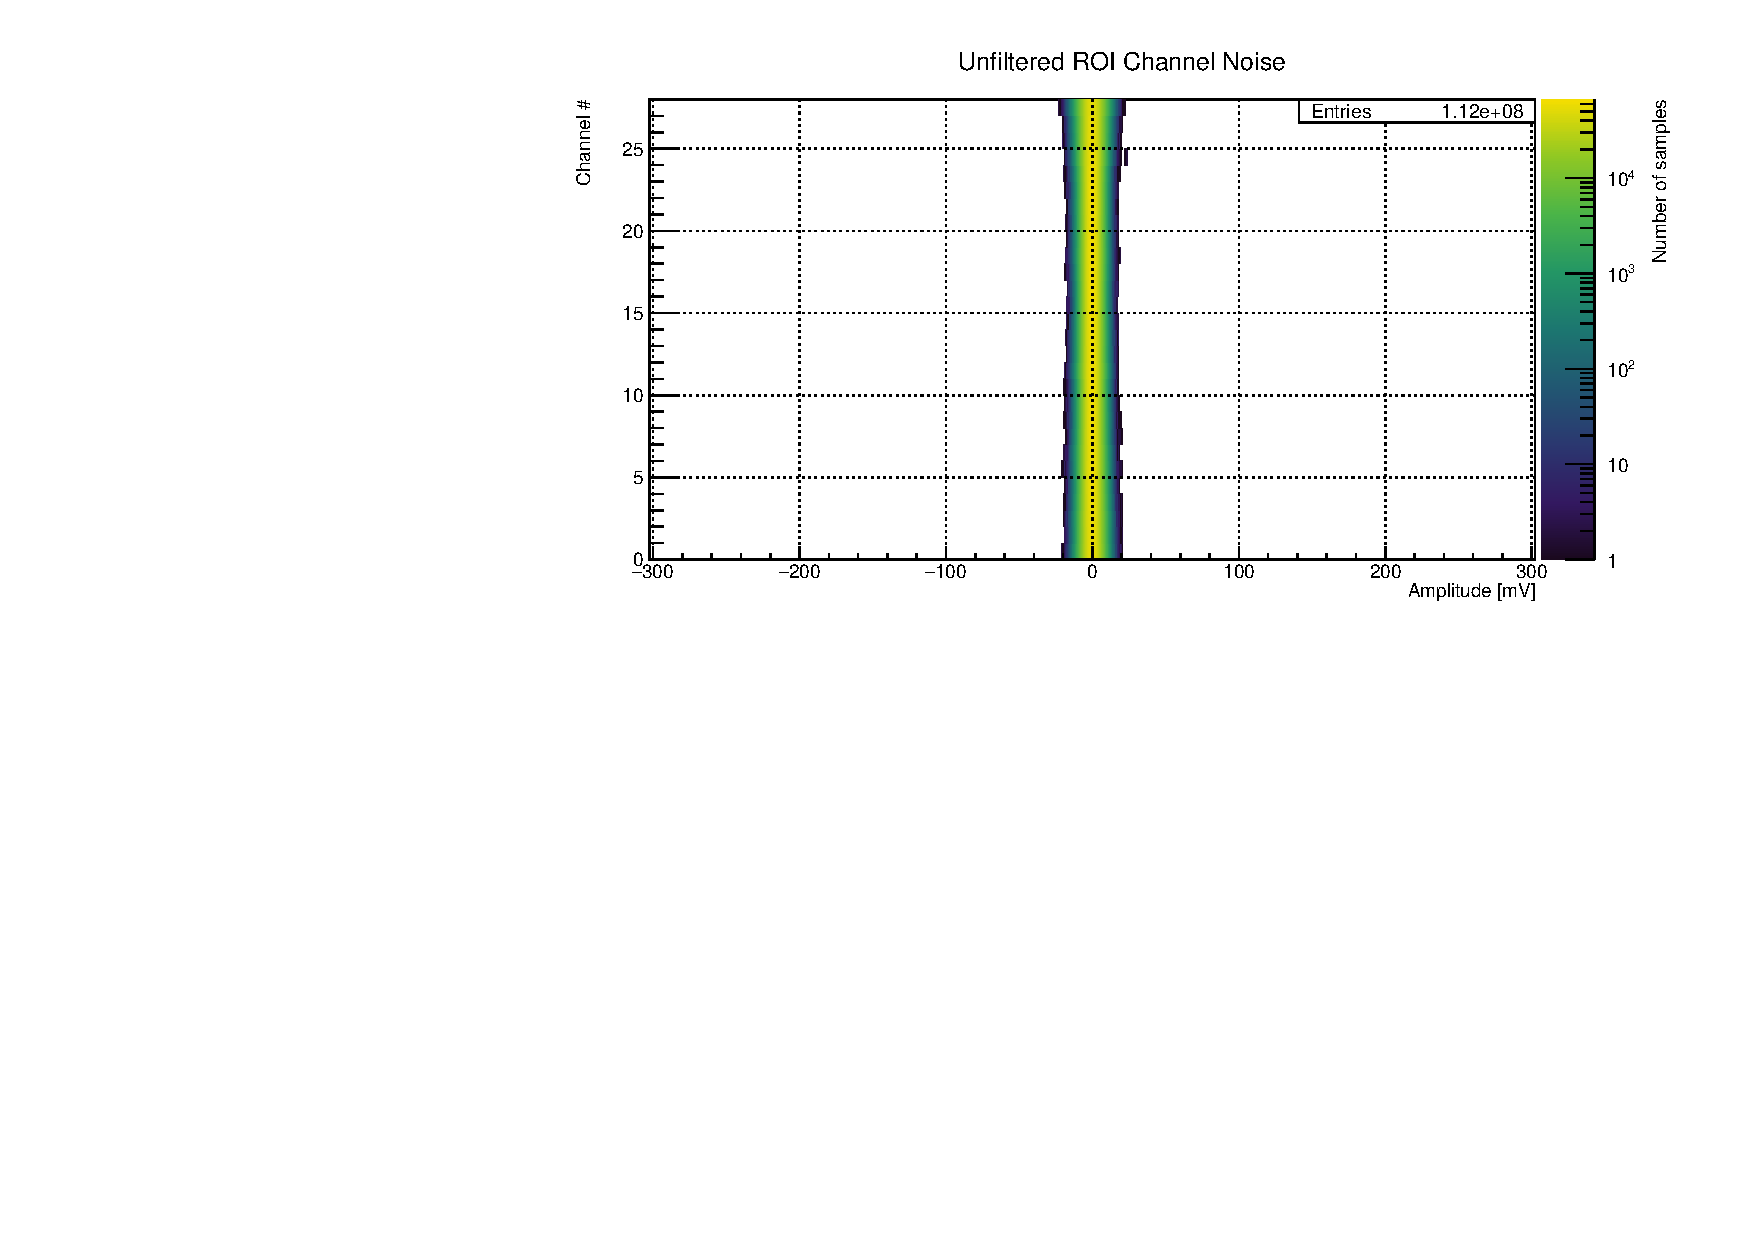
\includegraphics[page=1, width=\textwidth]{noise/noise_run2}
	\caption{Noise amplitude distributions of pixel (top) and ROI (bottom) channels of the second measurement campaign, after implementing hardware noise mitigation measures.
	\num{2000} events with \num{2000} \SI{210}{\nano\second} samples each from a \SI{5}{\hertz} random trigger were combined.}
	\label{fig:electronics_noise-run2}
\end{figure}

\afterpage{\clearpage}


\subsection*{Improved Cold Electronics for Pixelated Readouts}

This section describes the challenges met by electronics for pixelated \lartpc{}s and possible solutions.
First, the cryogenic Analogue-to-Digital Converters (ADCs) for the \dune{} far detector, developed by BNL, are introduced, and an explanation is given why they are unsuitable for a pixelated near detector.
Therefore, the neutrino group at Lawrence Berkeley National Laboratory (LBNL) is developing bespoke pixel electronics for the near detector, called \larpix{}.
An overview of this effort is given in the second part of this section.

As mentioned in Section~\ref{sec:lartpc_electronics}, cold digitisation can improve noise because of both shorter analogue signal lines and reduced thermal noise of the electronics.
Furthermore, it enables the multiplexing of the data on high-speed digital links, reducing the number of needed signal cables and cryostat feedthroughs.
However, designing reliable electronics at cryogenic temperatures is not an easy task.
ADCs in particular are very sensitive to stable reference voltages required for proper analogue-to-digital conversion.
Another problem arises from the fact that digital electronics in general require clocks with sharp edges for proper timing, usually realised as a square wave.
According to Fourrier analysis, a square wave produces a high level of harmonics.
This is particularly problematic in case of readout wires that act as antennas and can pick up theses clock signals.
A further important aspect is power dissipation.
All power dissipated by cryogenic electronics needs to be compensated for in order to prevent the \lar{} from boiling.
This is particularly problematic for a pixelated readout that requires a much higher number of readout channels than a wire readout (see Section~\ref{sec:studies_charge-ro}).

BNL is developing cold charge readout electronics for the \dune{} far detector.~\cite{protodune-sp}
In particular, the plan is to accompany the cryogenic LARASIC charge preamplifiers by cryogenic ADCs.
They have \num{16} inputs, each capable of digitising the TPC signals at \SI{2}{\mega{}S\per\second} and \SI{12}{bit} with input characteristics optimised for the LARASIC output.
A more detailed description is given in~\cite{bnl_adc}.

In the course of this work, the cryogenic ADC ASICs developed by BNL were evaluated to be used in the near detector as well.
The author joined the team at BNL in cold tests of the devices.
One of the results of these tests is presented here to illustrate the difficulties of cryogenic ADCs.
As a disclaimer, it should be noted that this is by no means the current status of the ADCs at the time of this writing.
The described tests were performed in the Fall of 2016 at BNL.

An important characteristic of an ADC is linearity.
It describes the relation between the applied input voltage and the calculated digital number, the \emph{ADC code}, at the output.
In the case of the BNL ADCs, this relation is expected to be strictly linear.
To test this, a voltage ramp is applied to the input and the converted digital values are recorded.

\begin{figure}[htb]
	\centering
	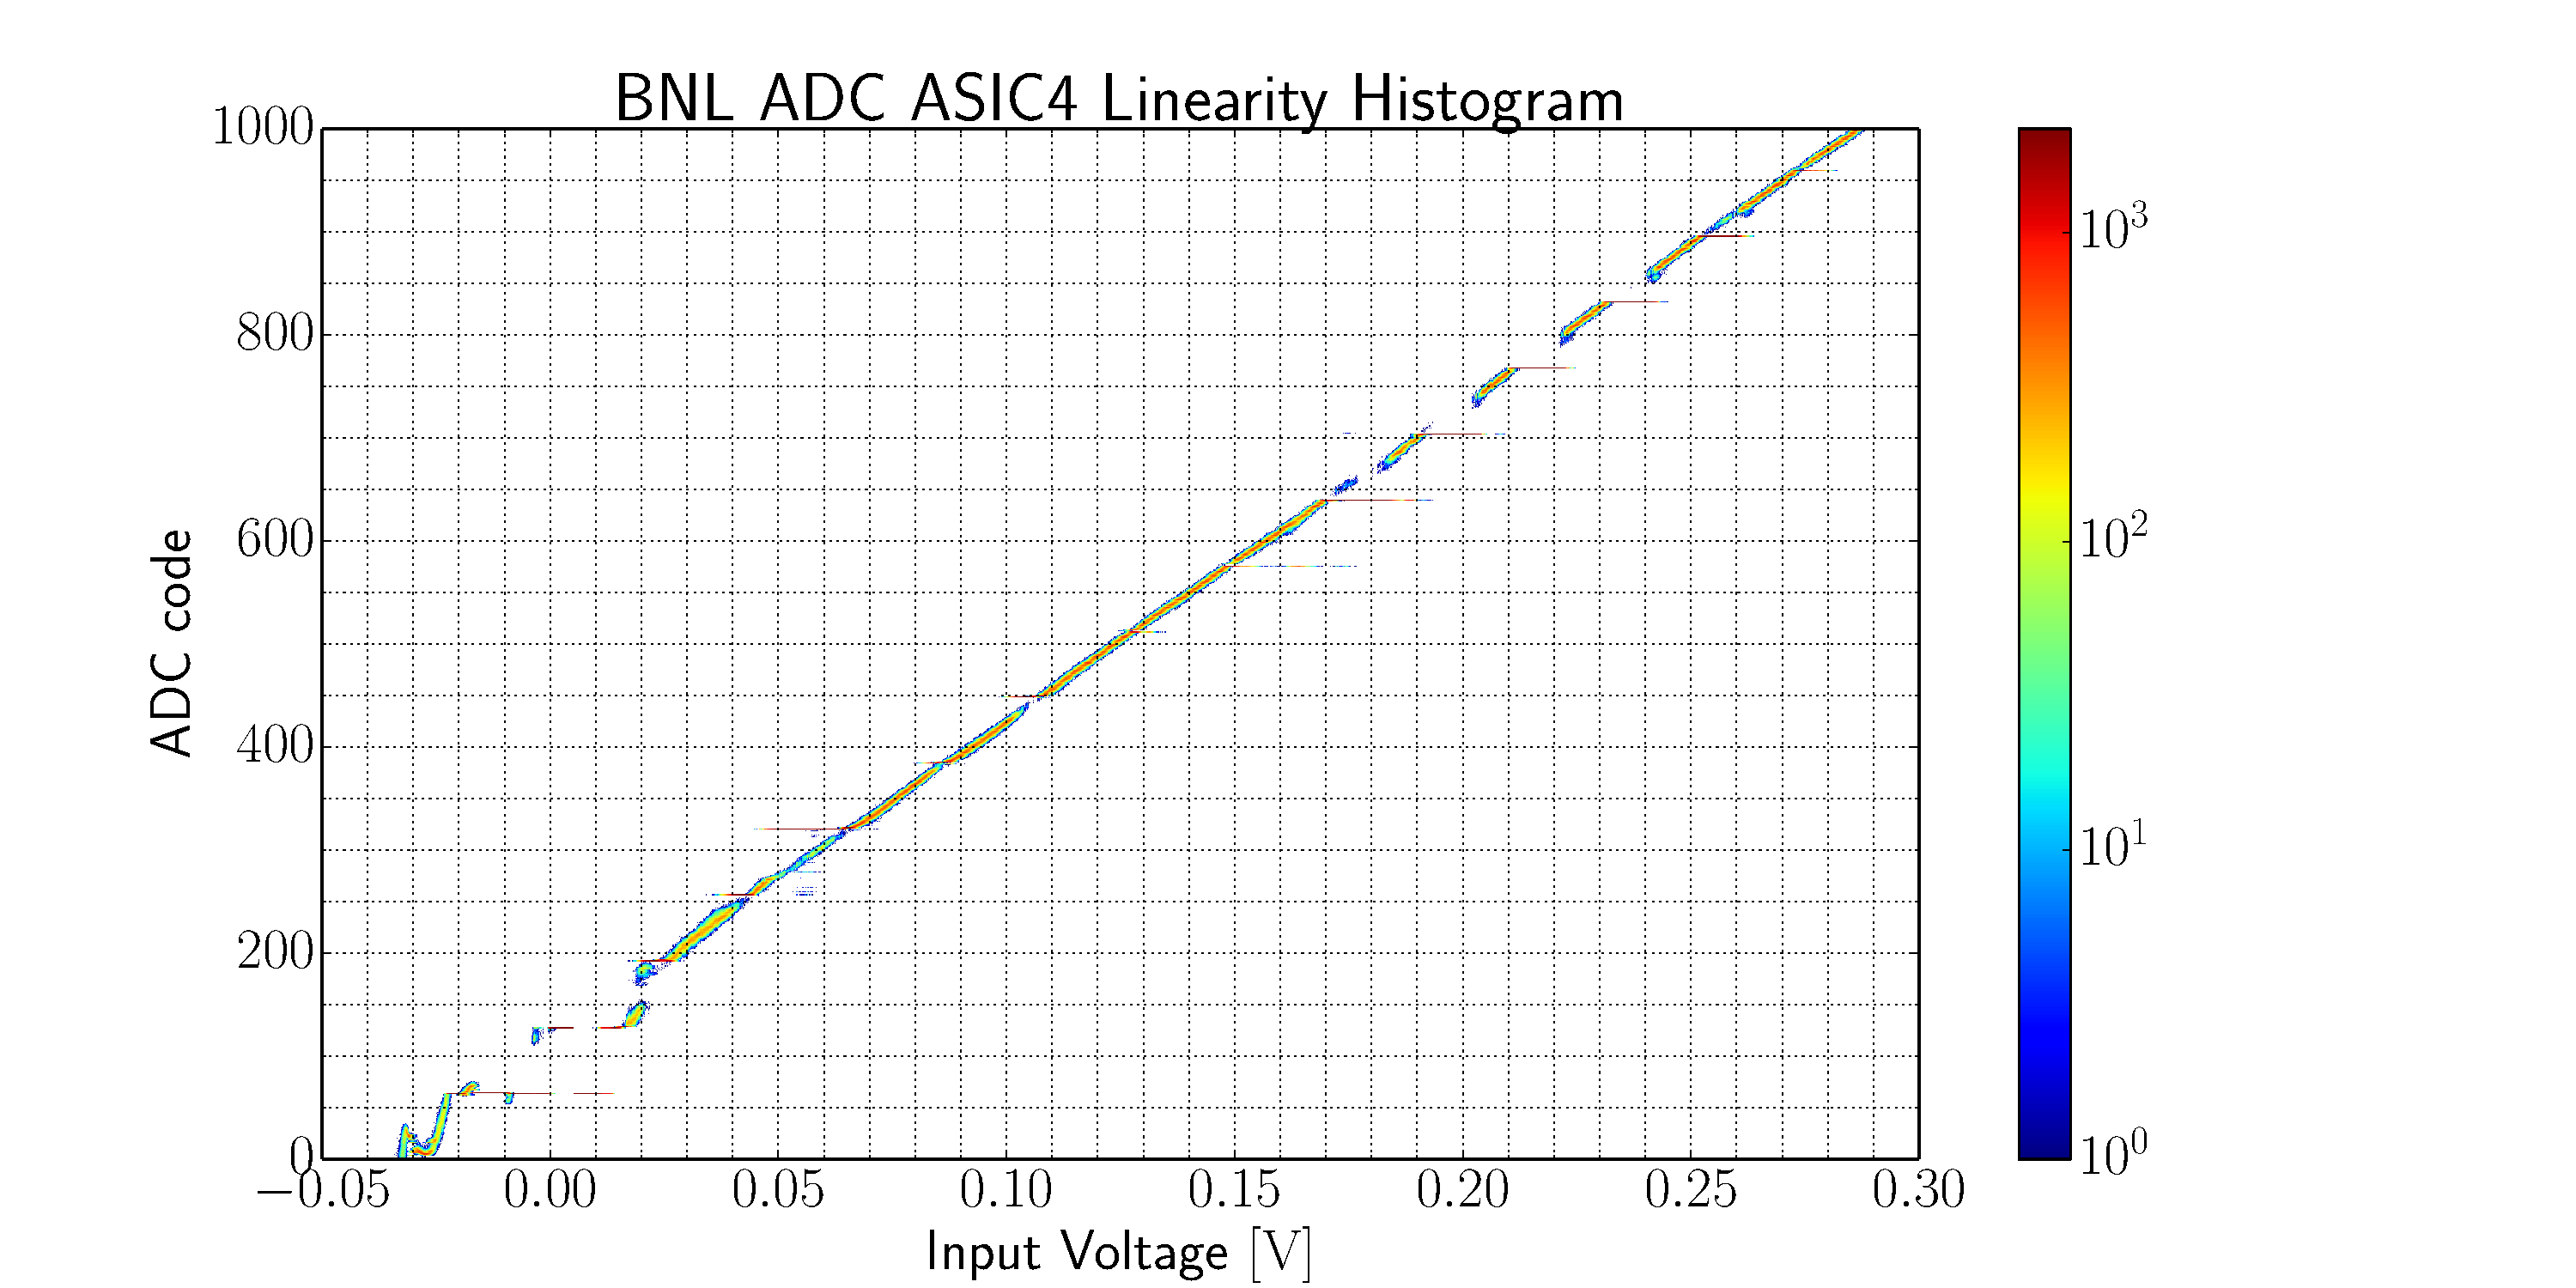
\includegraphics[width=\textwidth]{bnl/bnl_adc_lin}
	\caption{Linearity measurement of the BNL cryogenic ADC ASICs with input voltage on the x-axis and ADC value (code) on the y-axis.
	Color represents the number of measurements.
	The measurements were performed in liquid nitrogen.}
	\label{fig:bnl_adc_lin}
\end{figure}

A typical measurement is shown in Figure~\ref{fig:bnl_adc_lin}.
The expected shape is one straight diagonal line from the bottom left to the top right corner, i.e.\ a linear relationship between input voltage and ADC value.
Two particular deviations from this are visible: gaps accompanied by horizontal lines and a wobbly response around zero.
Upon close inspection, it can be seen that the gaps have the same voltage range as the horizontal lines.
The meaning of this is that for this input voltage range, the ADC output is \emph{stuck} at the same value.
Both these effects mean that the detector response to detected charge and thus energy deposition is not linear.
While some non-linearities can be compensated in offline data analysis, this is not possible for the sticking ADC values because they correspond to a range of input voltages.
This impairs the energy resolution of the detector.

The cause for the non-linearities is rooted in the electronic design of the ASIC.
Additionally, it was not fully understood at the time of these tests.
Therefore, an explanation is out of the scope of this work and not given here.
The measurements are shown to illustrate the difficulties of designing a reliable cryogenic ADC.

Leaving aside the non-linear response, the BNL ADC ASICs are not suitable for use in conjunction with a pixelated \lartpc{} charge readout.
Being designed for wire readouts, no strong focus was laid on power dissipation which is $\approx \SI{5}{\milli\watt}$ per channel.
Combined with the one of the LARASIC (\SI{10}{\milli\watt})~\cite{larasic}, a total of \SI{15}{\milli\watt} is dissipated.
For a pixelated \dune{} ND with $\order{\num{e7}}$ channels, the resulting required cooling power would be \SI{150}{\kilo\watt} for \SI{70}{\tonne} of \lar{} (see Section~\ref{sec:dune-nd_ac}).
In comparison, \uboone{} has a total cooling power of $\approx \SI{20}{\kilo\watt}$ for \SI{170}{\tonne} of \lar{}.~\cite{uboone}

Due to their smaller geometric extent, pixels have a much lower capacitance than wires.
According to Equation~\eqref{eq:electronics_thermal-noise}, this reduces the intrinsic noise present on a pixelated readout.
The \emph{\larpix{}} ASICs, being developed by LBNL~\cite{larpix}, exploits this fact to significantly reduce the complexity of the cold electronics.
Two key points distinguish them from the BNL design for the wire-equipped far detector.
The complex shaping preamplifier required by wires for noise filtering can be replaced by a simple charge integrator.
Additionally, the low noise levels allow for a self-triggering scheme; charge arriving at the \larpix{} is only digitised if it is above a prefedined thresholds.
This, in turn, reduces the duty cycle and thus the power dissipation of the ADC.
If noise levels are well below the set threshold, power dissipation becomes primarily a function of charge flux rate in the detector.

In addition to this, the digital circuitry of \larpix{} operates at lower frequencies than the BNL design.
For an alternating current (AC) of frequency $f$, the resistance presented by a conductor is not simply given by its Ohmic resistance.
There is an additional component proportional to $\sqrt{f}$ caused by the \emph{skin effect}.~\cite{horowitzHill}
High frequency currents no longer flow in the bulk of the conductor but only in a finite layer (skin) at its surface.
Therefore, the resistance is no longer proportional to the cross-section area but rather the surface area of the conductor.
The result of the skin effect is more power dissipation at higher frequencies.
By operating at lower frequencies, the power dissipation of \larpix{} can be lowered further.
The cost is a decrease in data transmission rates.

With its power dissipation (and comsumption) dependent on the charge flux and the lowered data transmission rate, \larpix{} is susceptible to high event rates.
Due to the triggered digitisation, the same goes for noise levels.
For the successful operation of \larpix{}, it is of paramount importance to keep event rates and noise levels low.
The latter can be achieved by minimising detector capacitance.
To lower the susceptibility to high event rates, the \dune{} ND design puts the TPC drift direction perpendicular to beam direction.
This reduces the amount of charge per event arriving simultaneously at the readout.
Furthermore, \larpix{} is equipped with a First-In-First-Out (FIFO) buffer capable of holding \num{2048} charge pulses to cope with short peaks in event rate.

To accomodate the elevated number of channels of a pixelated readout, the first \larpix{} prototype chip has \num{32} inputs.
Its resolution in time and charge are \SI{2}{\micro\second} and \SI{8}{bit}, respectively.
While currently inferior to the BNL design, these specifications are planned to be improved in the next design iteration, after a successful initial test.
One of the goals of the first prototype is to assess the optimal size of the FIFO.~\cite{danLarpix}

\afterpage{\clearpage}